\scanpage{53}
\margin{Avril 86}
\uline{Biicosaèdre \inserted{\uline{pas} \uline{\unsure{gauche|gauches}} \uline{et}} orientations}

Soit $(S,\{\deleted{\unsure{\Phi,\Phi'|\mathcal I,\mathcal I'}}\})$ un biicosaèdre \inserted{gauche} orienté, et soit
$\widetilde S_\Phi,\widetilde A_\Phi,\widetilde F_\Phi$ le revêtement \deleted{des} orienté de $(S,\Phi)$
$\widetilde S_{\Phi'},\widetilde A_{\Phi'},\widetilde F_{\Phi'}$ celui de $(S,\Phi')$.
\inserted{Ce sont des icos. ``droits'' orientés.} On va définir des
bijections
\[
\begin{aligned}
\varepsilon^S_{\Phi',\Phi\deleted{\unsure{'}}}&:\widetilde S_\Phi\mathrel{\overset{\sim}{\longrightarrow}}\deleted{\widetilde A}\widetilde S_{\Phi'}\\
\varepsilon^A_{\Phi',\Phi\deleted{\unsure{'}}}&:\widetilde A_\Phi\mathrel{\overset{\sim}{\longrightarrow}}\deleted{\unsure{\widetilde S}}\widetilde A_{\Phi'}\\
\varepsilon^F_{\Phi',\Phi\deleted{\unsure{'}}}&:\widetilde F_\Phi\mathrel{\overset{\sim}{\longrightarrow}}\widetilde F_{\Phi'}
\end{aligned}
\]
\margin{(voir rectification, il faut remplacer $\widetilde A_\Phi,\widetilde A_{\Phi'}$ par $\overline A_\Phi$ et $\overline A_{\Phi'}$, ens des arêtes \uline{orientées})}
comme voici.

\deleted{\unsure{$\widetilde S_\Phi$}} La fibre de $\widetilde S_\Phi$ et $\widetilde S_{\Phi'}$ en un point $s\in S$ sont les
deux \inserted{\deleted{\unsure{deux}} ens. des orientations des deux} structures pentagonales sur $S\smallsetminus\{s\}$ associées
\deleted{de} l'une à $\Phi$, l'autre à $\Phi'$, et qui sont associées. \deleted{Elles}
ont $=$ groupe des rotations, \inserted{$U_s$}, \deleted{\unsure{isomorphe}} qui
est un \deleted{espace aff.} $\mathbb F_5$-module libre de rang $1$,
et $U_s^*$ (ens des générateurs) est un torseur sous le groupe cyclique
$\mathbb F_5^*$ \inserted{iso à $\mathbb Z/4\mathbb Z$}, \deleted{\unsure{leurs}}
\deleted{par \illegible{2} l'élément $2$}
\margin{On voit $U_s^*$ \unsure{s'identifiant|distinguer} \unsure{longueur} de}
\figure{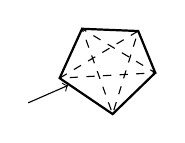
\begin{tikzpicture}[scale=.57]
\coordinate (a) at (0,.1);\coordinate (b) at (.5,1.2);\coordinate (c) at (1.75,1.15);\coordinate (d) at (2.13,.22);\coordinate (e) at (1.18,-.70);
\draw[thick] (a)--(b)--(c)--(d)--(e)--cycle;
\draw[dashed] (a)--(c)--(e)--(b)--(d)--cycle;
\draw[->] (-.7,-.45)--(.19,-.06);
\end{tikzpicture}}
% slanted: note beside the pentagon
$(\widetilde S_\Phi)_s$ est l'une des classes modulo le sous-groupe $\pm1$
soit $\{u,-u\}$, et $\widetilde S_{\Phi',s}$ est l'autre classe, donc
$\{2u,\deleted{\unsure{u}}-2u\}$.

L'application
\[
\varepsilon^S_{\Phi,\Phi'}(s):\widetilde S_\Phi(s)\longrightarrow\widetilde S_{\Phi'}(s)
\quad\text{est donnée par}\quad
u\longmapsto 2u
\]
On aura
\[
\deleted{\unsure{\varepsilon}}\varepsilon_{\Phi',\Phi\deleted{\unsure{'}}}(s)
\deleted{\unsure{\varepsilon}}\varepsilon^{\deleted{\unsure{2a|S}}}_{\Phi,\Phi'}(s)
=\deleted{\unsure{a}}u\longmapsto4u=-u=\underline a_{\Phi'}u
\]
($\underline a_{\Phi'}$ l'antipodisme de $\Phi'$,
et de $=$ en sens inverse. (Si on avait choisi
$u\mapsto3u$\inserted{$=-2u$}, ça aurait été pareil, car
$\inserted{3^2=(-2)^2}\deleted{\unsure{4}}\equiv-1\ (5)$)
\deleted{\unsure{tout comme} $4\equiv-1\ (5)$)} Donc
% slanted
\margin{On a \unsure{l'iso} can (indépendt du choix de $\Phi$ dans $\{\Phi,\Phi'\}$) $\widetilde S_{\Phi(s)}\unsure{\times|\wedge}\widetilde S_{\Phi'}(s)\simeq\{\Phi,\Phi'\}$ les deux choix différant par $\underline a_\Phi$ (ou $\underline a_{\Phi'}$) \deleted{On voit \unsure{ainsi}}}
\[
\left\{\begin{aligned}
\varepsilon_{\Phi',\Phi}\varepsilon_{\Phi,\Phi'}&=a_{\Phi'}\qquad\text{et de }=\\
\varepsilon_{\Phi,\Phi'}\varepsilon_{\Phi',\Phi}&=a_\Phi
\end{aligned}\right.
\tag*{(1)}
\]
\margin{donc l'identification entre $\widetilde S_\Phi$ et $\widetilde S_{\Phi'}$ dépend du choix d'un $\Phi$ ou de $\Phi'$, dans $\{\Phi,\Phi'\}$}

Soit une face $t$ de $\Phi$, $t'$ sa complémentaire, face de $\Phi'$.
on a une bijection canonique
\[
\alpha^{\deleted{\unsure{S}}}_{\Phi',\Phi}:\unsure{t'_\Phi|t_\Phi}\simeq t_{\Phi'}\quad \deleted{\unsure{t}}\quad
\text{(et $\alpha_{\Phi,\Phi'}$ est l'inverse !)}
\]
d'où
\[
\varepsilon^F_{\Phi',\Phi}:
\underset{\substack{\Vert\\\widetilde A_{\Phi,t}}}{\omega(t_\Phi)}
\xrightarrow{\sim}\underset{\substack{\Vert\\\widetilde A_{\Phi',t'}}}{\omega(t_{\Phi'})}
\]
% archive sheet number: 52
